\section{Further analysis on the effect of sequence length} \label{2506:app:further-sequence-length}
The aim of this Appendix is to clarify and give further examples on Theorem~\ref{2506:thm:sequencelength-gain}. Here we provide an intuitive explanation of the result, while the mathematical details can be found in Appendix~\ref{2506:app:proofs}. 

\subsection{Anatomy of the gain}
The gain counts \emph{gradient steps} (Definition~\ref{2506:def:weak-recovery}), while the analysis of Appendix~\ref{2506:app:proofs} is carried out on the gradient flow of Equation~\eqref{2506:eq:ode_approx}, which lives in continuous time. The learning rate is what converts one into the other, and it is precisely this conversion that decides whether the sequence length enters the gain once or twice. In this Appendix we write \(t_\mathrm{tied}\) and \(t_\mathrm{untied}\) for the weak recovery times of the gradient flow, and keep \(\nu^\mathrm{weak}_\eta\) for the number of gradient steps.\addnote{Appendix~\ref{2506:app:proofs} uses the opposite letters: what is called \(\nu_\eta\) and \(\nu_{\eta,\mathrm{untied}}\) there is written \(t_\mathrm{tied}\) and \(t_\mathrm{untied}\) here, while its \(t^+_\eta\) is a number of gradient steps.}

\paragraph{From continuous time to gradient steps}
Theorem~\ref{2506:thm:app:ben_arous_meta} relates the two, for a network whose gradient flow reaches weak recovery at time \(t\). As long as the learning rate obeys
\begin{equation} \label{2506:eq:app:gamma-max}
    \gamma \lesssim \gamma^\mathrm{max} \sim \frac{1}{d\,t},
\end{equation}
weak recovery is reached after
\begin{equation} \label{2506:eq:app:steps-from-flow}
    \nu^\mathrm{weak}_\eta \sim \frac{t}{\gamma}
\end{equation}
gradient steps, whereas above \(\gamma^\mathrm{max}\) the inhibitive term of Equation~\eqref{2506:eq:ode_approx} dominates at initialization and the network never leaves the uninformative region. The key observation is that \(t\) appears in \emph{both} equations: saturating Equation~\eqref{2506:eq:app:gamma-max} gives \(\nu^\mathrm{weak}_\eta \sim d\,t^2\), so the weak recovery time of the flow is paid twice when the learning rate is itself scaled up with \(L\), and only once when it is held fixed. This is the whole origin of the two regimes discussed below.

\paragraph{The two weak recovery times}
Close to initialization, both networks follow a flow of the same shape (Appendix~\ref{2506:app:proofs}),
\begin{equation} \label{2506:eq:app:generic-flow}
    \frac{dm}{dt} \sim \alpha\, m^{\mathrm{SIE}-1},
\end{equation}
and differ only through the drift constant \(\alpha\) and the threshold \(\theta\) that the overlap has to reach:
\begin{equation} \label{2506:eq:app:drift-threshold}
    \begin{aligned}
        \alpha_\mathrm{tied} &= C_\mathrm{SIE} \times (\vec{1},\dots,\vec{1}), &\qquad \theta_\mathrm{tied} &= \eta, \\
        \alpha_\mathrm{untied} &= \norm{C_\mathrm{SIE}}_\mathrm{op}, &\qquad \theta_\mathrm{untied} &= \eta\sqrt{L}.
    \end{aligned}
\end{equation}
The drifts differ because of the structure of the two networks: the tied network builds up correlation faster than the untied one, since its single weight vector composes the \(L\) signals of the sequence coherently and therefore feels the target through its contraction along \((\vec{1},\dots,\vec{1})\); the untied network, having \(L\) independent weights, can only follow the leading direction of the tensor \(C_\mathrm{SIE}\), whose strength is measured by the operator norm. The thresholds differ for a purely geometric reason: weak recovery of the untied network is expressed through \(m_\mathrm{untied} = \sfrac{\norm{\vec{m}}}{\sqrt{L}}\), so its overlap \emph{vector} has to reach a norm \(\sqrt{L}\) times larger than the scalar overlap of the tied network.

Integrating Equation~\eqref{2506:eq:app:generic-flow} from the initial overlap \(m(0) \sim \sfrac{1}{\sqrt{d}}\) up to \(\theta\) gives
\begin{equation} \label{2506:eq:app:hitting-times}
    t \sim \frac{1}{\alpha}\cdot\begin{cases}
        \theta & \mathrm{SIE} = 1,\\
        \ln d & \mathrm{SIE} = 2,\\
        d^{\frac{\mathrm{SIE}}{2}-1} & \mathrm{SIE} \ge 3,
    \end{cases}
\end{equation}
and this is where the special role of \(\mathrm{SIE}=1\) is born. When \(\mathrm{SIE}=1\) the overlap grows linearly in time, so the weak recovery time is directly proportional to the threshold, and a threshold \(\sqrt{L}\) times larger costs exactly \(\sqrt{L}\) times more time. When \(\mathrm{SIE}\ge 2\) the growth is instead exponential (\(\mathrm{SIE}=2\)) or explosive (\(\mathrm{SIE}\ge 3\)), and the weak recovery time is dominated by the escape from the small initial overlap \(m(0)\): the threshold then enters only logarithmically, or through a bounded additive term, and its \(\sqrt{L}\) is subleading. Dividing the two hitting times,
\begin{equation} \label{2506:eq:app:flow-ratio}
    \frac{t_\mathrm{untied}}{t_\mathrm{tied}} \sim \frac{C_\mathrm{SIE} \times (\vec{1},\dots,\vec{1})}{\norm{C_\mathrm{SIE}}_\mathrm{op}} \cdot \begin{cases}
        \sqrt{L} & \mathrm{SIE} = 1,\\
        1 & \mathrm{SIE} \ge 2.
    \end{cases}
\end{equation}

\paragraph{Why the factor for \(\mathrm{SIE}=1\) is sometimes \(\sqrt{L}\) and sometimes \(L\)}
Writing Equation~\eqref{2506:eq:app:steps-from-flow} for both networks, the gain splits into two factors,
\begin{equation} \label{2506:eq:app:gain-breakdown}
    \mathrm{gain} = \frac{\nu^\mathrm{weak}_{\eta,\mathrm{untied}}}{\nu^\mathrm{weak}_\eta} \sim \frac{t_\mathrm{untied}}{t_\mathrm{tied}} \cdot \frac{\gamma_\mathrm{tied}}{\gamma_\mathrm{untied}},
\end{equation}
and everything hinges on how the two learning rates are chosen. If the networks are trained with the same learning rate --- or, more generally, with two rates whose ratio does not scale with \(L\) --- the second factor is \(1\). If instead each network is given the largest learning rate it can afford, Equation~\eqref{2506:eq:app:gamma-max} turns the second factor into a second copy of the first, because \(\gamma_\mathrm{tied}^\mathrm{max}/\gamma_\mathrm{untied}^\mathrm{max} = t_\mathrm{untied}/t_\mathrm{tied}\). Hence
\begin{equation} \label{2506:eq:app:gain-two-regimes}
    \mathrm{gain} \sim \begin{cases}
        \dfrac{t_\mathrm{untied}}{t_\mathrm{tied}} & \text{equal learning rates},\\[2.5ex]
        \left(\dfrac{t_\mathrm{untied}}{t_\mathrm{tied}}\right)^{2} & \text{optimal learning rates}.
    \end{cases}
\end{equation}
Substituting Equation~\eqref{2506:eq:app:flow-ratio} in the second case gives
\begin{equation} \label{2506:eq:app:gain-optimal}
    \mathrm{gain} \sim \left(\frac{C_\mathrm{SIE} \times (\vec{1},\dots,\vec{1})}{\norm{C_\mathrm{SIE}}_\mathrm{op}}\right)^{2} \cdot \begin{cases}
        L & \mathrm{SIE} = 1,\\
        1 & \mathrm{SIE} \ge 2,
    \end{cases}
\end{equation}
which is exactly the statement of Theorem~\ref{2506:thm:sequencelength-gain}: the theorem is formulated at the optimal learning rate, as announced when the gain was defined. The extra factor attached to \(\mathrm{SIE}=1\) is therefore \emph{not} a constant of the model: it is \(\sqrt{L}\) when the two networks share the same learning rate, and \(L\) when both rates are pushed to their maximum. It is one and the same effect --- the \(\sqrt{L}\) larger threshold of Equation~\eqref{2506:eq:app:drift-threshold} --- counted once or twice, exactly like the drift ratio next to it.

For later use, combining Equations~\eqref{2506:eq:app:gamma-max} and~\eqref{2506:eq:app:hitting-times}, the largest admissible learning rates scale with the sequence length as
\begin{equation} \label{2506:eq:app:gamma-max-scalings}
    \begin{aligned}
        \gamma_\mathrm{tied}^\mathrm{max} &\propto C_\mathrm{SIE} \times (\vec{1},\dots,\vec{1}),\\
        \gamma_\mathrm{untied}^\mathrm{max} &\propto \norm{C_\mathrm{SIE}}_\mathrm{op}\cdot\begin{cases}
            \sfrac{1}{\sqrt{L}} & \mathrm{SIE} = 1,\\
            1 & \mathrm{SIE} \ge 2,
        \end{cases}
    \end{aligned}
\end{equation}
up to factors that do not depend on \(L\). Their ratio is again \(t_\mathrm{untied}/t_\mathrm{tied}\), as it must be.

\subsection{Example at non-optimal learning rate}
In Figure~\ref{2506:fig:sequence-length-H2} we presented the speed up in the case of a target function with \(\mathrm{SIE}=2\), and optimal learning rate for both the tied and untied network. Here we want to show that our result predicts the gain well even when the learning rates are not scaled up optimally. In particular, consider the same setting as in Figure~\ref{2506:fig:sequence-length-H2}, but with the learning rates
\begin{equation}
    \gamma_\mathrm{tied} = \gamma_\mathrm{untied} = \gamma_0 \qquad\text{independent of } L.
\end{equation}
The target is \(g(\vec{z}_\star)= \sum_{i=1}^L \mathrm{He}_2(z_{\star,i})\), so that \(C_2 = I_L\), \(C_2 \times (\vec{1},\vec{1}) = L\) and \(\norm{C_2}_\mathrm{op} = 1\). Since \(\mathrm{SIE}=2\) there is no threshold correction, and Equation~\eqref{2506:eq:app:flow-ratio} gives \(t_\mathrm{untied}/t_\mathrm{tied} \sim L\). The two learning rates are equal, so we are in the first case of Equation~\eqref{2506:eq:app:gain-two-regimes} and the flow ratio is counted only once:
\begin{equation}
    \mathrm{gain} \sim \frac{t_\mathrm{untied}}{t_\mathrm{tied}} \sim L.
\end{equation}
\begin{figure}
    \centering
    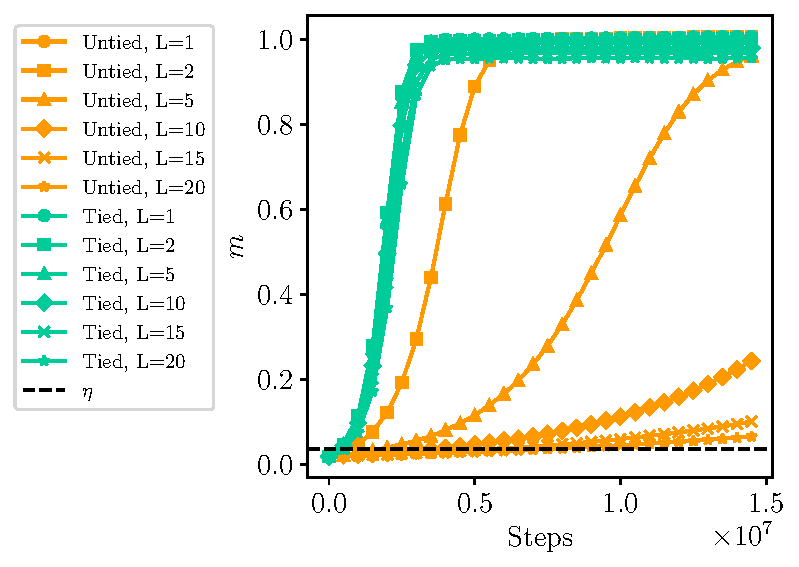
\includegraphics[height=0.27\textwidth]{figs/sequence-lenght/H2-sequence-length-icoverlapped-overlap}
    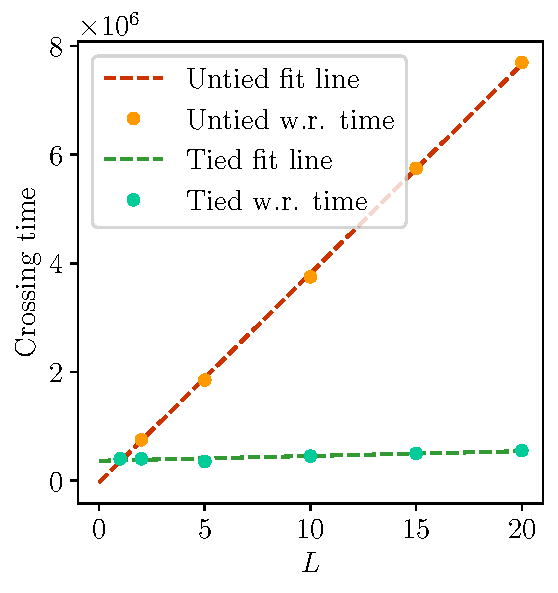
\includegraphics[height=0.27\textwidth]{figs/sequence-lenght/H2-sequence-length-icoverlapped-crossing}
    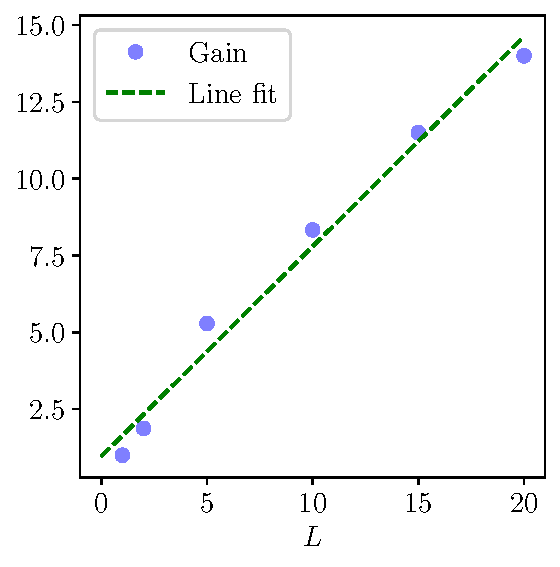
\includegraphics[height=0.27\textwidth]{figs/sequence-lenght/H2-sequence-length-icoverlapped-gain}
    \caption{The gain in the case of a target function with \(\mathrm{SIE}=2\), where both cases use the same learning rate \(\gamma_0 = 0.005\). (left) The evolution of the overlap, (middle) the weak recovery time and (right) the gain. The gain is proportional to \(L\), as predicted. \(d=3000\), \(\sigma=\ReLU\)}
    \label{2506:fig:app:sequence-length-H2_costantlrate}
\end{figure}
In Figure~\ref{2506:fig:app:sequence-length-H2_costantlrate} we show the result of the simulation, where we can see that the gain is indeed proportional to \(L\), as predicted. It is worth stressing that this is the very same target function as in Figure~\ref{2506:fig:sequence-length-H2}, where the measured gain is instead \(L^2\): the two experiments differ only in the choice of the learning rates, which decides whether the flow ratio is counted once or twice.

\subsection{The upper bound on the learning rate scaling}
In this subsection we want to show an example proving that not all scalings of the learning rate are allowed: if it grows too fast with the sequence length, the network will not be able to learn.

Let's take as example the \(\mathrm{SIE}=1\) target function
\begin{equation}
    g(\vec{z}_\star) = \frac{1}{\sqrt{L}}\sum_{i=1}^L z_{\star,i},
\end{equation}
with the corresponding leading Hermite tensor
\begin{equation}
    C_1 = \begin{pmatrix}
        \sfrac{1}{\sqrt{L}} & \dots & \sfrac{1}{\sqrt{L}}
    \end{pmatrix} \in \mathbb{R}^{L},
\end{equation}
for which \(C_1 \times \vec{1} = \sqrt{L}\) and \(\norm{C_1}_\mathrm{op} = 1\). This time \(\mathrm{SIE}=1\), so the threshold correction of Equation~\eqref{2506:eq:app:flow-ratio} is active and contributes a second \(\sqrt{L}\):
\begin{equation} \label{2506:eq:app:H1-flow-ratio}
    \frac{t_\mathrm{untied}}{t_\mathrm{tied}} \sim \frac{C_1 \times \vec{1}}{\norm{C_1}_\mathrm{op}} \cdot \sqrt{L} = \sqrt{L}\cdot\sqrt{L} = L.
\end{equation}
We train both networks with one and the same \(L\)-independent learning rate
\begin{equation}
    \gamma_\mathrm{tied} = \gamma_\mathrm{untied} = \gamma_0,
\end{equation}
so that, once again, the flow ratio is counted only once:
\begin{equation}
    \mathrm{gain} \sim \frac{t_\mathrm{untied}}{t_\mathrm{tied}} \sim L.
\end{equation}
\begin{figure}
    \centering
    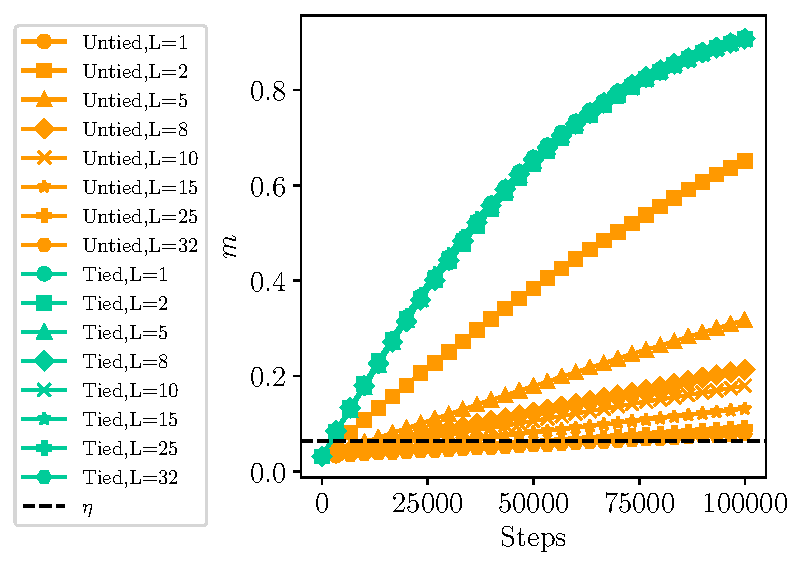
\includegraphics[height=0.27\textwidth]{figs/sequence-lenght/H1-sequence-length-icoverlapped-overlap}
    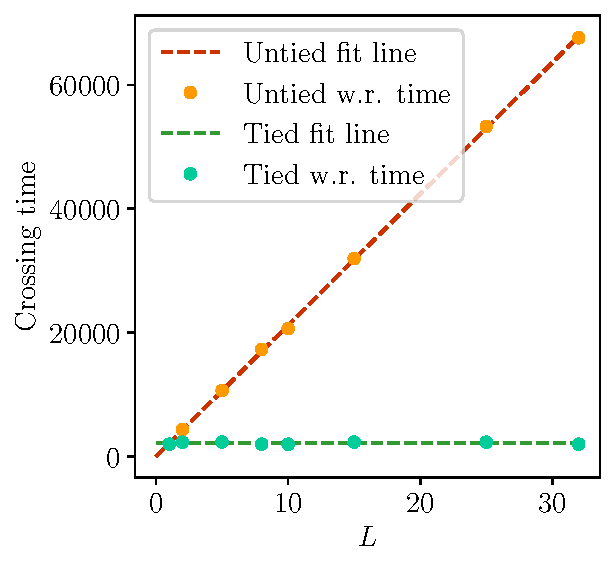
\includegraphics[height=0.27\textwidth]{figs/sequence-lenght/H1-sequence-length-icoverlapped-crossing}
    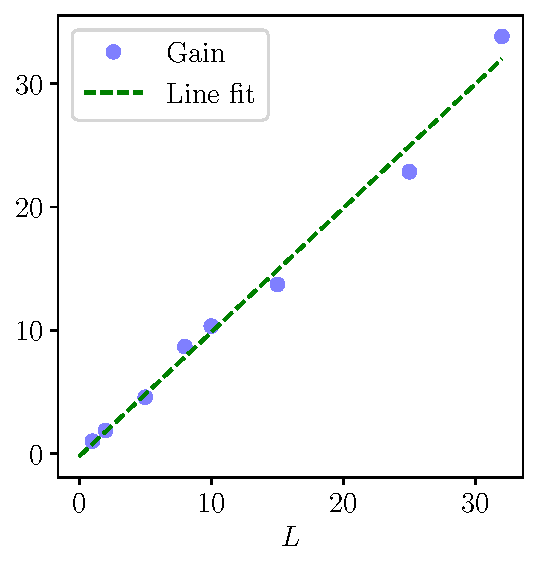
\includegraphics[height=0.27\textwidth]{figs/sequence-lenght/H1-sequence-length-icoverlapped-gain}
    \caption{The gain in the case of a target function with \(\mathrm{SIE}=1\), where both cases use the same learning rate \(\gamma_0 = 0.015\). (left) The evolution of the overlap, (middle) the weak recovery time and (right) the gain. The gain is proportional to \(L\), as predicted. \(d=1000\), \(\sigma=\ReLU\)}
    \label{2506:fig:app:sequence-length-H1_base}
\end{figure}
In Figure~\ref{2506:fig:app:sequence-length-H1_base} we show the result of the simulation, where we can see that the gain is indeed proportional to \(L\), as predicted. Note that here the \(\mathrm{SIE}=1\) correction shows up as a \(\sqrt{L}\), and not as the \(L\) of Theorem~\ref{2506:thm:sequencelength-gain}, precisely because the learning rates are held fixed: had we instead scaled both of them up to their maximum, Equation~\eqref{2506:eq:app:gain-optimal} would have predicted \(\mathrm{gain} \sim (\sqrt{L})^2 \cdot L = L^2\). The two experiments of this Appendix therefore both measure a gain proportional to \(L\), but for different reasons: for \(\mathrm{SIE}=2\) the whole factor comes from the drift ratio, while for \(\mathrm{SIE}=1\) half of it comes from the drift ratio and half from the larger threshold of the untied network.

We can now ask what happens if we push the learning rate scaling of the untied network beyond the limit of Theorem~\ref{2506:thm:sequencelength-gain}. If we keep \(\gamma_\mathrm{tied} = \gamma_0\) and set
\begin{equation}
  \gamma_\mathrm{untied} = \gamma_0 \cdot L,
\end{equation}
the ratio between the learning rates becomes now \(\sfrac{\gamma_\mathrm{tied}}{\gamma_\mathrm{untied}} = \sfrac{1}{L}\), and Equation~\eqref{2506:eq:app:gain-breakdown} would give
\begin{equation}
  \mathrm{gain} \sim L \cdot \frac{1}{L} = 1.
\end{equation}
Apparently, the untied network performance is matching the one of the tied network. The prediction is however void, because Equation~\eqref{2506:eq:app:steps-from-flow} only holds below the threshold of Equation~\eqref{2506:eq:app:gamma-max}: for this target the largest admissible rate of the untied network \emph{decreases} with the sequence length as \(\sfrac{1}{\sqrt{L}}\), by Equation~\eqref{2506:eq:app:gamma-max-scalings}, so a learning rate growing as \(\gamma_0 L\) overshoots it by a factor \(L^{\sfrac{3}{2}}\). Figure~\ref{2506:fig:app:sequence-length-H1_maxlrate} shows the result of the simulation of such a case: the learning rate of the untied network is too high, the untied network stops reaching weak recovery as \(L\) grows, and the measured gain diverges instead of settling to a constant. This plot proves our bounds on the learning rate scaling are indeed correct.
\begin{figure}
  \centering
  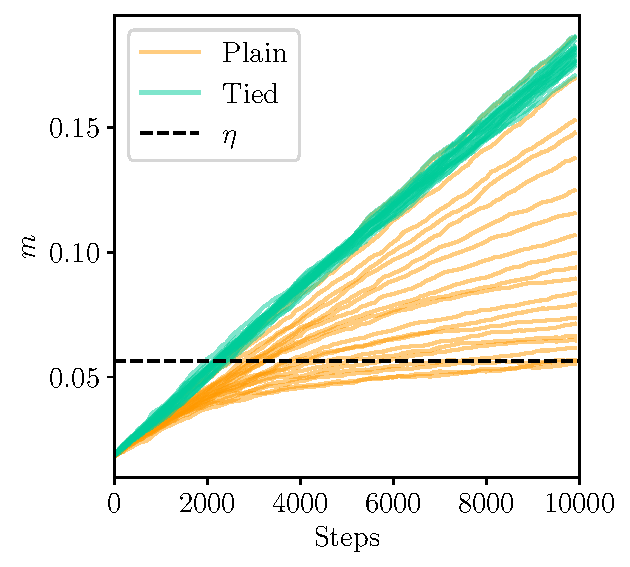
\includegraphics[height=.3\textwidth]{figs/sequence-lenght/H1-sequence-length-maxlr-overlap}
  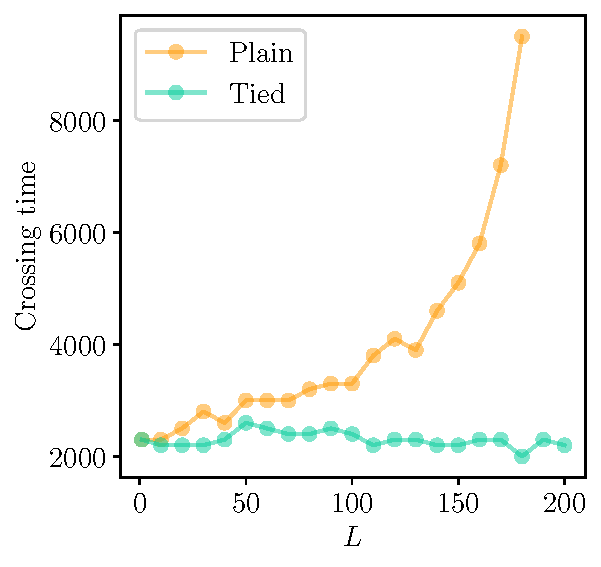
\includegraphics[height=.3\textwidth]{figs/sequence-lenght/H1-sequence-length-maxlr-crossing}
  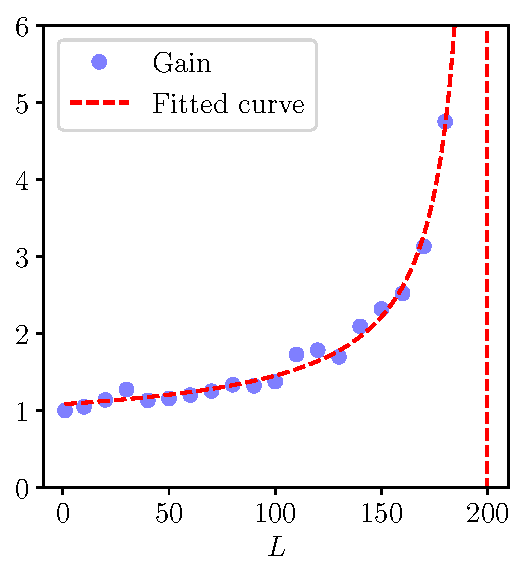
\includegraphics[height=.3\textwidth]{figs/sequence-lenght/H1-sequence-length-maxlr-gain}
  \caption{The gain in the case of a target function with \(\mathrm{SIE}=1\), where the untied network is trained with \(\gamma_\mathrm{untied} = \gamma_0 L\), beyond the bound of Equation~\eqref{2506:eq:app:gamma-max}, while the tied one keeps \(\gamma_\mathrm{tied} = \gamma_0 = 0.05\). (left) The evolution of the overlap, (middle) the weak recovery time and (right) the gain. The gain diverges, as predicted. \(d=3000\), \(\sigma=\ReLU\)}
  \label{2506:fig:app:sequence-length-H1_maxlrate}
\end{figure}


\subsection{Equivalence between Single-Layer attention and Tied network}
\begin{figure}
    \centering
    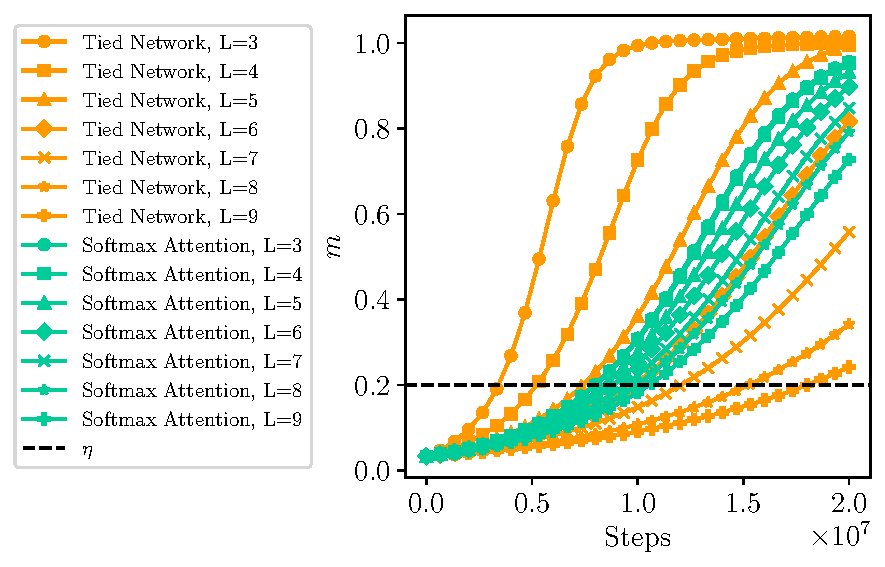
\includegraphics[height=0.3\textwidth]{figs/sequence-lenght/comparison-attention-squarenetwork-overlap}
    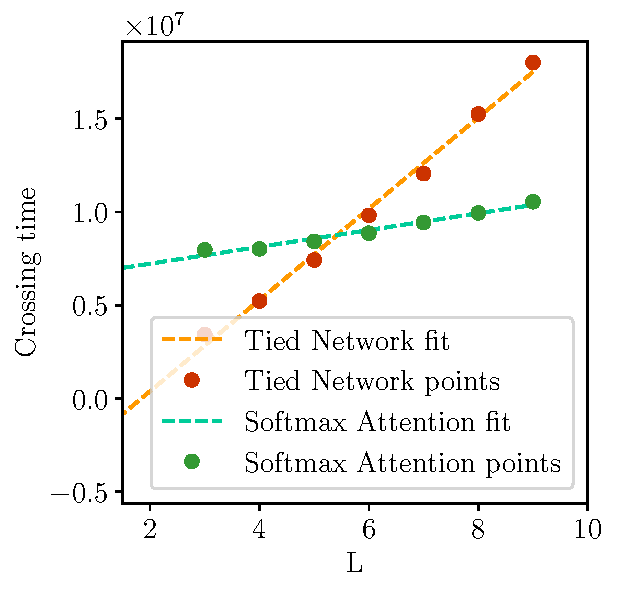
\includegraphics[height=0.3\textwidth]{figs/sequence-lenght/comparison-attention-squarenetwork-crossing}
    \caption{Comparison between the learning of the tied network with squared activation (orange), namely linear attention, and the single-layer softmax attention (green). (left) The evolution of the overlap; each symbol is a different value of \(L\). (right) the weak recovery time. The two networks learn at the same rate, but with different constants. \(g(\vec{z}_\star)=\sum_{i=1}^L\mathrm{He}_2(\vec{z}_{\star,i})\), \(d=1000\), \(\sigma=\ReLU\)}
    \label{2506:fig:app:attention-squarenetwork}
\end{figure}
In the main paper we proved that the tied network model is a generalization of the single-layer attention model. In particular, if the activation function is  \(\sigma(x) = x^2\), the tied network is equivalent to the single-layer \emph{linear} attention. We also claimed that adding a non-linearity to the attention can only improve the performance of the network, although not affecting the scaling with the sequence length. In Figure~\ref{2506:fig:app:attention-squarenetwork} we show the comparison between the learning of the tied network with squared activation (orange), namely linear attention, and the single-layer softmax attention(green). The two networks learn at the same linear rate, but with different growth constants. Softmax attention performs better than the tied network with squared activation for sufficiently large sequence lengths.




\subsection{Pathological cases}
Theorem~\ref{2506:thm:sequencelength-gain} shows that there could be cases where the gain from learning is 0, meaning that the tied network cannot learn anything, while the untied one possibly can. In particular the degenerate condition happens when
\begin{equation}
    C_\mathrm{SIE} \times (\vec{1},\dots,\vec{1}) = 0,
\end{equation}
where Theorem~\ref{2506:thm:sequencelength-gain} guarantees that the gain is 0. Examples of such pathological cases are:
\begin{itemize}
    \item \(\mathrm{SIE}=1\): a possible pathological target could be
          \[
            g(\vec{z}_\star) = z_{\star,1} - z_{\star,2}.
          \]
          In this case the leading term in Hermite expansion is
          \[
            C_1 = \begin{pmatrix}
                1\\ 
                -1
            \end{pmatrix} \quad \text{and consequently } C_1 \times \vec{1} = 0.
          \]
    \item \(\mathrm{SIE}=2\): analogously, a possible pathological target could be
          \[
            g(\vec{z}_\star) = z^2_{\star,1} - z^2_{\star,2}.
          \]
            In this case the leading term in Hermite expansion is
            \[
            C_2 = \begin{pmatrix}
                1 & 0\\ 
                0 & -1
            \end{pmatrix} \quad \text{and consequently } C_2 \times \begin{pmatrix} 1& 1\\ 1& 1\end{pmatrix} = 0.
            \]
\end{itemize}
In Figure~\ref{2506:fig:app:degenerate} we show the pathological case for \(\mathrm{SIE}=1\) and \(\mathrm{SIE}=2\). The untied network is not able to learn the target function because of the symmetry: the tied network is by design symmetric, while the target is constructed to be as antisymmetric as possible in the sequence length. The untied network instead is able to learn the target function, because the weights are not constrained to be equal, thus the symmetry is broken by the initialization. 
\begin{figure}
    \centering
    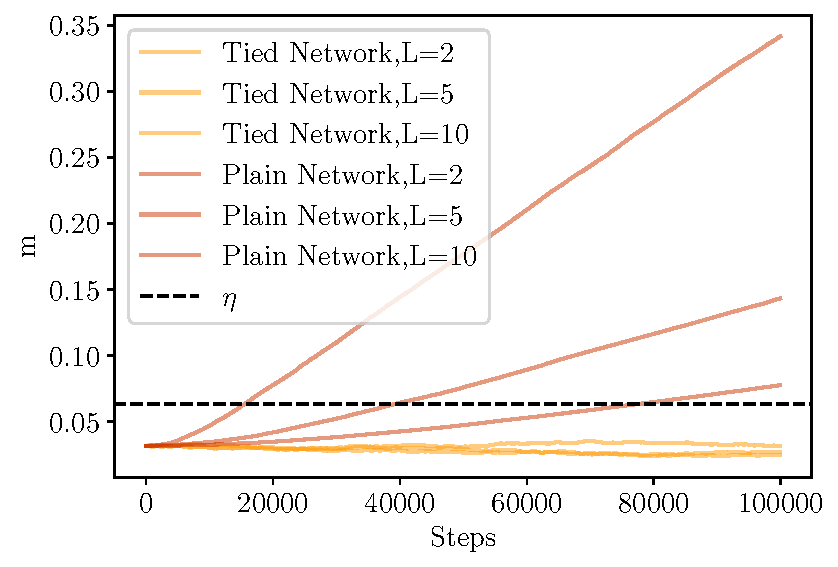
\includegraphics[width=0.45\textwidth]{figs/sequence-lenght/degeneracy_nulldivergence}
    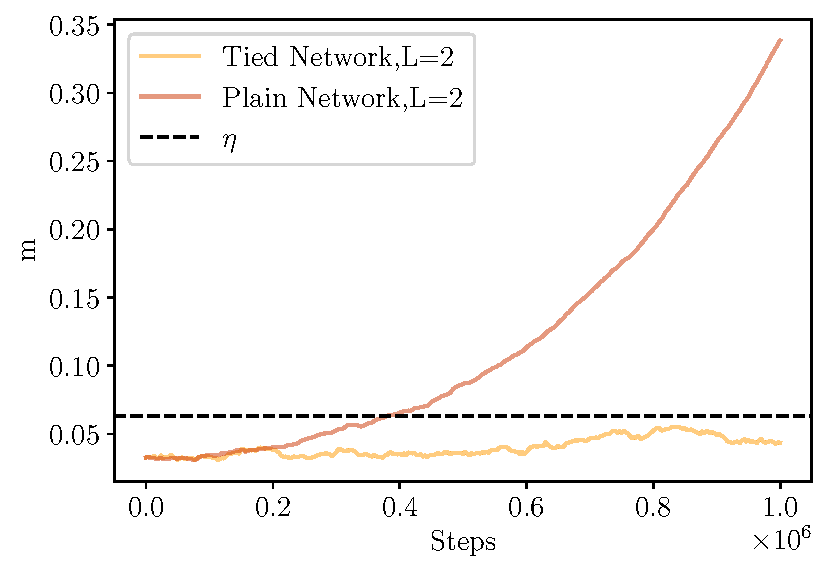
\includegraphics[width=0.45\textwidth]{figs/sequence-lenght/degeneracy_nulldivergence-v2}
    \caption{Pathological cases for \(\mathrm{SIE}=1\) (left) and \(\mathrm{SIE}=2\) (right). The untied network is able to learn the target function, while the tied one cannot.}
    \label{2506:fig:app:degenerate}
\end{figure}

The degeneracy of the tied network could be solved by weighting randomly the neurons. In that case, almost surely we have
\begin{equation}
    C_\mathrm{SIE} \times (\vec{1},\dots,\vec{1}) \neq 0.
\end{equation}
Although this is a possible solution, we leave the study of the effect of random weights for symmetry breaking for future work.
